\documentclass{article}
\usepackage[utf8]{inputenc}
\usepackage{CJKutf8} % 用来支持中文
\usepackage{caption}
\usepackage{graphics}
\usepackage{array}
\usepackage{booktabs}
\usepackage{geometry}
\usepackage{amsmath} % 用来写数学公式
\geometry{left=3.2cm, right=3.2cm, top=2.0cm, bottom=2.0cm}
\usepackage{setspace}
\setstretch{1.2} 
\usepackage[colorlinks,linkcolor=blue]{hyperref}
\usepackage{amsthm}
\usepackage{amsfonts}
\usepackage{graphicx}
\usepackage{epstopdf}
\setcounter{secnumdepth}{0} % section不显示编号
\usepackage{color}
\definecolor{shadecolor}{rgb}{0.94, 0.94, 1.0}
\usepackage{framed}
\newcommand{\RNum}[1]{\uppercase\expandafter{\romannumeral #1\relax}}  % 罗马数字
\usepackage{bm}  % 数学字母粗体并保持斜体的格式

\title{\textbf{Statistical Inference Assignment 9}}
\author{Junhao Yuan (20307130129)}
\date{\today}

\begin{document}
\begin{CJK}{UTF8}{gbsn}

    \maketitle
    \def \RR{{\mathbb R}}
    \def \EE{{\mathbb E}}
    \def \VV{{\mathbb V}}
    \def \II{{\mathbb I}}
    \def \NN{{\mathcal N}}


    % Problem 1
    \begin{shaded}
        \noindent\textsc{Problem 1.}\par
        Suppose $X_1, \ldots, X_{20}\mathop{\sim}\limits^{iid}B(p)$. We want to test the hypothesis
        \begin{align}
            H_0: p=0.2\qquad vs\qquad  H_1: p \neq 0.2.\label{power-1}
        \end{align}
        Suppose the decision rule is $\phi(\bm{x})$ and $\phi(\bm{x})=1$ if and only if $\sum_{i=1}^{20} x_i \geq 7$ or
        $\sum_{i=1}^{20} x_i \leq 1$.
        \begin{itemize}
            \item [(a)] Find the power of the decision rule when $p=0,\, 0.1,\, 0.2, \ldots, 0.9$. Draw
                  a graph of the power as a function of $p$.
            \item [(b)] Find the type \RNum{1} error probability of the rule $\phi$. What is the type \RNum{2} error
                  probability when $p=0.05$?
        \end{itemize}
    \end{shaded}
    \noindent\textsc{Solution.}\par
    \begin{itemize}
        \item [(a)]
              The power of the decision rule can be computed by:
              \begin{align}
                  \beta(p) & = (1-p)^{20} + 20 p(1-p)^{19} + \sum_{k=7}^{20} p^k (1-p)^{20-k}.\notag
              \end{align}
              And the result is shown below:
              \begin{figure}[htbp]
                  \centering
                  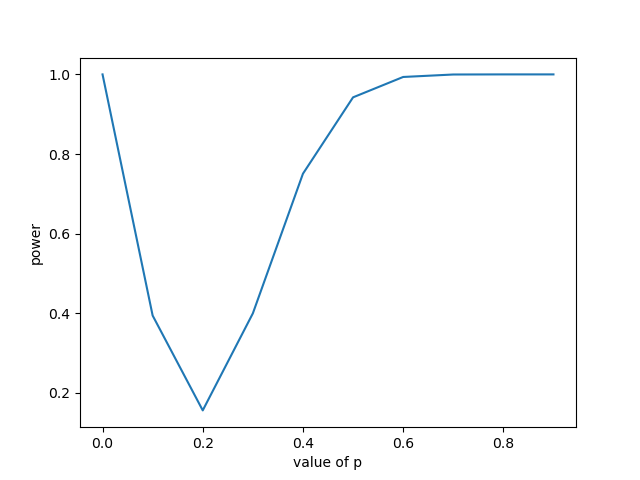
\includegraphics[scale=0.4]{power.png}
                  \label{power}
              \end{figure}

        \item [(b)]
              By the calculation results in problem (a), we can know that the type \RNum{1} error probability is $\beta(0.2)\approx 0.156$.

              When $p=0.05$, by \eqref{power-1}, we have $\beta(0.05)\approx 0.736$. Therefore, the type \RNum{2}
              error probability is $1-\beta(0.05)\approx0.264$.
    \end{itemize}






    % Problem 2
    \begin{shaded}
        \noindent\textsc{Problem 2.}\par
        Suppose $X_1, \ldots, X_{10}\mathop{\sim}\limits^{iid} U(0, \theta)$. Construct a test for testing
        \begin{align}
            H_0: \theta \leq 1 \qquad vs \qquad H_a: \theta \geq 1
        \end{align}
        at a level $\alpha$ (Construct a test means finding a rejection region).
    \end{shaded}
    \noindent\textsc{Solution.}\par
    Intuitively, we can use $X_{(n)}$ to estimate $\theta$, and $X_{(n)}/\theta \sim Beta(n, 1)$. Under $H_0$, we
    have $X_{(n)} \sim Beta(n, 1)$. Suppose there exists a $c$ such that
    \begin{align}
        P(X_{(n)} > c) = \alpha, \notag
    \end{align}
    then a level $\alpha$ rejection region is $(\, c, +\infty\,)$. Since $P(X_{(n)} > c) \mathop{=}\limits^{H_0} 1 - c^{n}$, we have
    $c = (1 - \alpha)^{1/n}$, which means the rejection region with level $\alpha$ is $(\, (1 - \alpha)^{1/n}, +\infty)$. In this
    problem, it's $(\, (1 - \alpha)^{1/10}, +\infty)$.
    Therefore, when $X_{(10)}$ is grater than $(1-\alpha)^{1/n}$, we can reject the null hypothesis. Otherwise, we can not
    reject it.



    % Problem 3
    \begin{shaded}
        \noindent\textsc{Problem 3.}\par
        Suppose $X_1, \ldots, X_n\mathop{\sim}\limits^{iid}U(0, \theta)$. Use $\max\,\{ X_i\}_{i=1}^n$ to find a
        $(1-\beta, 1-\gamma)$ tolerance interval.
    \end{shaded}
    \noindent\textsc{Problem 3.}\par
    Suppose there exists a $\lambda$ such that
    \begin{align}
        P_{\theta}(P^*_{\theta}(\lambda X_{(n)} \leq X \leq X_{(n)})\geq 1-\beta) \geq 1 - \gamma.\label{3}
    \end{align}
    Since
    \begin{align}
        P_{\theta}^* (\lambda X_{(n)} \leq X \leq X_{(n)}) = (1-\lambda) \frac{X_{(n)}}{\theta},\notag
    \end{align}
    where $X_{(n)}/\theta \sim Beta(n, 1)$, we can rewrite \eqref{3} as
    \begin{align}
        P_{\theta} \left (\frac{X_{(n)}}{\theta}\geq \frac{1-\beta}{1-\lambda}\right ) \geq 1-\gamma.\notag
    \end{align}
    Let $Y=X_{(n)}/\theta \sim Beta(n, 1)$ with cdf $F(y)=y^n$.Then we have
    \begin{align}
        P_{\theta} \left (\frac{X_{(n)}}{\theta}\geq \frac{1-\beta}{1-\lambda}\right )  = 1 - F\left (\frac{1-\beta}{1-\lambda} \right ) \geq 1-\gamma.\notag
    \end{align}
    We can let
    \begin{align}
        1 - F\left (\frac{1-\beta}{1-\lambda} \right )  = 1 - \left (\frac{1-\beta}{1-\lambda} \right )^n= 1-\gamma,\notag
    \end{align}
    which gives us a reasonable value of $\lambda$:
    \begin{align}
        \lambda_0 =1 - \frac{1-\beta}{\gamma^{1/n}}.\notag
    \end{align}
    Therefore, one $(1-\beta, 1-\gamma)$ tolerance interval is
    \begin{align}
        [\,\lambda_0 X_{(n)},\,\, X_{(n)}\,].\notag
    \end{align}



\end{CJK}
\end{document}